\renewcommand{\ldate}{2016-01-12}
% 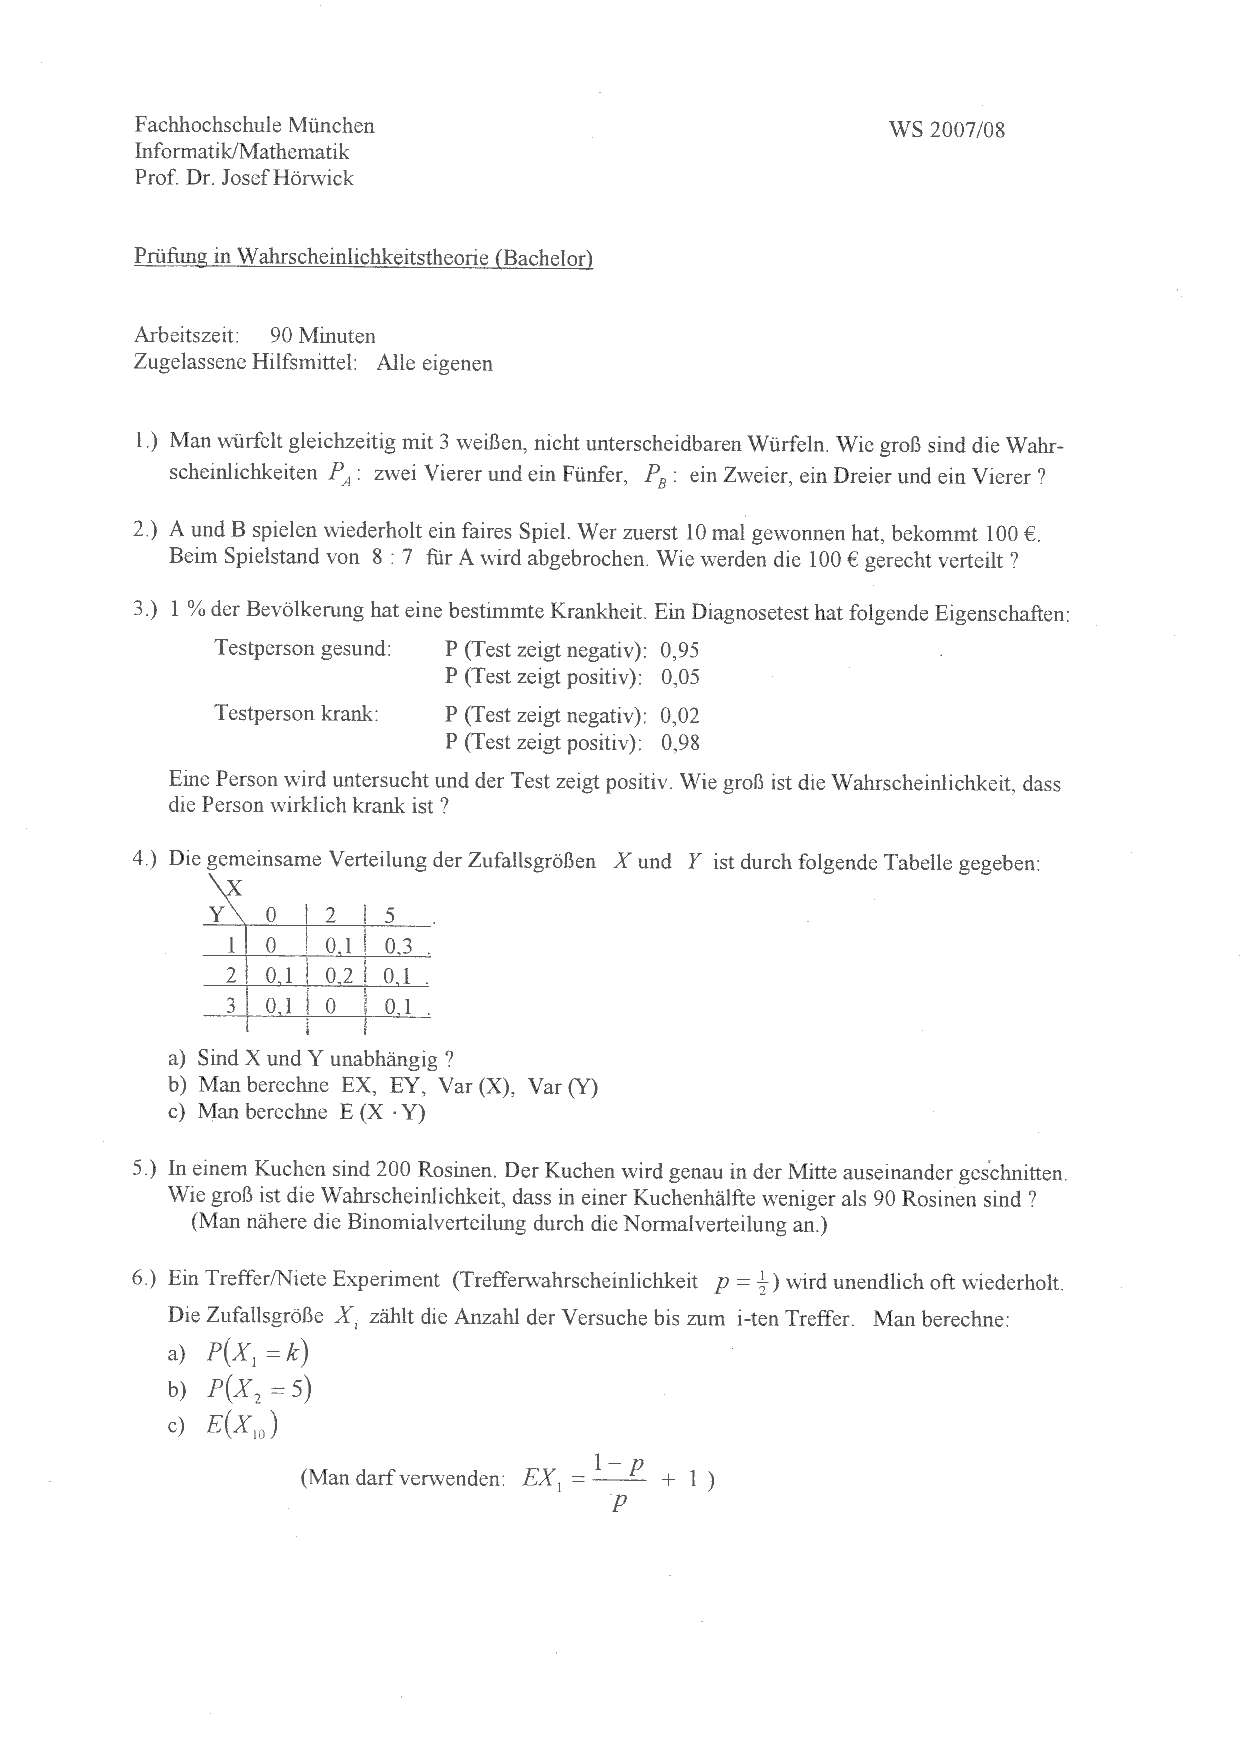
\includepdf[pages=-]{pruefungsangabe_wahrStat_ws0708}

\section{Lösung für die Prüfung WS 2007/08}

\subsection{zu 1)}
Wir stellen uns die Würfel verschiedenfarbig vor, dann ist es leichter (rot, grün, weiß). 

Alle Möglichkeiten: $ 6^3 = 216 $. Jede Möglichkeit ist gleich wahrscheinlich.

Günstige Möglichkeiten $P_A$: 

\begin{tabular}{|c|c|c|}
\hline r & g & w \\ 
\hline 5 & 4 & 4 \\ 
\hline 4 & 5 & 4 \\ 
\hline 4 & 4 & 5 \\ 
\hline 
\end{tabular}  
$\Rightarrow 3$ Möglichkeiten
$\Rightarrow P_A = \frac{3}{216} = 0.0138...$

Günstige Möglichkeiten $P_B$: 

\begin{tabular}{|c|c|c|}
\hline r & g & w \\ 
\hline 2 & 3 & 4 \\ 
\hline 2 & 4 & 3 \\ 
\hline 3 & 2 & 4 \\ 
\hline 3 & 4 & 2 \\ 
\hline 4 & 2 & 3 \\ 
\hline 4 & 3 & 2 \\ 
\hline 
\end{tabular}  
$\Rightarrow 6$ Möglichkeiten
$\Rightarrow P_A = \frac{6}{216} = 0.0277...$

\subsection{zu 2)}
Wie groß ist die Wahrscheinlichkeit, dass A beim Spielstand 8:7 gewinnt? Wir stellen uns vor, dass die beiden noch vier mal Spielen. Wir schreiben uns alle Spielausgänge hin. Diese sind gleich wahrscheinlich (halbe halbe). \color{red} A gewinnt \color{blue} B gewinnt. 

\color{red}

A A A A\\
B A A A\\
A B A A\\
A A B A\\
A A A B\\

\color{black}
Jetzt gewinnt jeder zweimal:
\color{red}

B B A A\\ 
B A B A\\
B A A B\\
A B B A\\
A B A B\\
A A B B\\
\color{black}
Jetzt gewinnt B dreimal: 
\color{blue}

A B B B\\
B A B B\\
B B A B\\
B B B A\\
B B B B\\
\color{black}
$P(\textrm{A gewinnt}) = \frac{11}{16} $ A bekommt $ 100 \textrm{ EUR} \cdot \frac{11}{16} = 68.75 \textrm{ EUR}$

\subsection{zu 3)}
Siehe Prüfung SS 2012

\subsection{zu 4)}
Siehe Prüfung SS 2012

\subsection{Exkurs: Annäherung der Binomialverteilung durch die Normalverteilung}
\profnote{Neuer Stoff für Aufgabe 5.}
Die zufallsgröße S sei $Bin(n,p)$ verteilt. Wir haben ein Treffer-Niete-Experiment mit der Trefferwahrscheinlichkeit p, das n mal wiederholt wird. S zählt die Anzahl der Treffer (0 bis n).\\

$P(S=k) = \binom n k \cdot p^k \cdot q^{n-k} $ mit $ q = 1-p, k=0,1,...,n, ES = np, Var(S)=npq $\\

Wir standardisieren S:

$ S^* = \frac{S - ES}{\sqrt{Var(S)}} $, wobei $S^*$ den Erwartungswert 0 und die Varianz 1 hat. 

$ x_j = \frac{j - np}{\sqrt{npq}}, j=0,1,...,k $\\

$ S^* $ kann die Werte $x_j$ annehmen. 

$ P (S^* = x_j) = P(S=j) $

Abstand von $x_{j+1}$ und $x_j$ ist mit $\frac{1}{\sqrt{npq}}$ immer gleich. \\

Zeichne von $S^*$ das Histogramm: Dazu zeichnen wir über $x_j$ ein Rechteck mit der Breite $\frac{1}{\sqrt{npq}}$ und Fläche $P(S^* = x_j) $.\\

Höhe des Rechtecks über $x_j$: $ \frac{1}{npq} \cdot h_j = P(S^* = x_j) = \binom n j \cdot p^j \cdot q^{n-j} $\\

% 1 \includegraphicsdeluxe{histogrammWS0708ex.jpg}{Histogramm}{So könnte das Histogramm aussehen}{fig:histogrammWS0708ex}
Man kann zeigen: Für große n nähert sich das Histogramm der Gaußschen Glockenkurve an (Abb. \ref{fig:histogrammWS0708ex}):
$ \varphi(x) = \frac{1}{\sqrt{2\pi}} \cdot exp\rbr{-\frac{x^2}{2}}$ Dabei ist $\varphi(x) $ die Dichte der Normalverteilung. 

$ \Phi(t) = \int_{-\infty}^{t} \varphi(x) dx$. $ \Phi(t)$ ist die Stammfunktion von $\varphi(x)$, kann aber nicht als Formel angegeben werden. Es gibt nur eine Tabelle. \\

Es gilt:
\begin{enumerate}
\item $ \int_{-\infty}^{\infty} \varphi(x) dx = 1$
\item $ \int_{-\infty}^{0} \varphi(x) dx = \frac{1}{2}, \varphi$ ist symmetrisch zur y-Achse.
\item $ \Phi(-t) = 1 - \Phi(t) \Rightarrow $ Wir brauchen die Tabelle nur für positive Werte. 
\end{enumerate} 

Damit kann man die Binomialverteilung durch die Normalverteilung annähern. 

S ist binomialverteilt $Bin(n,p)$

$ P(a \leq S \leq b) 
= P \rbr{\underbrace{\frac{a-np}{\sqrt{npq}}}_{u} \leq \underbrace{\frac{S-np}{\sqrt{npq}}}_{S^*} \leq \underbrace{\frac{b-np}{\sqrt{npq}}}_{v}}
= P( u\leq S^* \leq v)
\approx \int_{u}^{v} \varphi(x) dx = \Phi(v) - \Phi(u) 
$ (noch ungenau).

% 2-3 \includegraphicsdeluxe{besserWSRechtecke.jpg}{Histogramm}{Histogramm: u und v}{fig:besserWSRechtecke}
Beim ersten und letzten Rechteck fehlt eine Hälfte (Abb. \ref{fig:besserWSRechtecke}), deshalb besser: 

$P \rbr{\underbrace{\frac{a - \frac{1}{2} - np}{\sqrt{npq}}}_{u} \leq S^* \leq \underbrace{\frac{b + \frac{1}{2} - np}{\sqrt{npq}}}_{v} }$

\subsection{zu 5)}
L ist die linke Kuchenhälfte

X ist die Anzahl der Rosinen in L.

X ist binomialverteilt: $ n = 200, p=0.5 $

$ P(X < 90) + P(X > 110) $

Gegenereignis: 

$ P(90 \leq X \leq 110) $ mit $ EX = np = 200 \cdot 0.5 = 100 $ und $ Var(X) = npq = 200\cdot 0.5 \cdot 0.5 = 50 \Rightarrow $ 
$ P(90 \leq X \leq 110) 
= P\rbr{\frac{90 - 0.5 - 100}{\sqrt{50}} \leq X^* \leq \frac{110 + 0.5 - 100}{\sqrt{50}} }
= P(-1.48 \leq X^* \leq 1.48)
\approx \int_{-1.48}^{1.48} = \Phi(1.48) - \Phi(-1.48) 
= \Phi(1.48) - \underbrace{[1-\Phi(1.48)]}_{\textrm{Formel!}}
= 2 \cdot \Phi(1.48) -1 
= 2\cdot 0.93056 - 1 = $
\underline{$0.86...$}

Die gesuchte Wahrscheinlichkeit (wir haben ja das Gegenereignis ausgerechnet) ist damit $1-0.86...= 0.14$

\subsection{zu 6)}
Siehe Prüfung SS 2012